\documentclass[a4paper, 14pt]{extarticle}
\usepackage{geometry}

\usepackage{cmap} % Улучшенный поиск русских слов в полученном pdf-файле
\usepackage{mathtext} % русские буквы в формулах
\defaulthyphenchar=127 % Если стоит до fontenc, то переносы не впишутся в выделяемый текст при 
%копировании его в буфер обмена
\usepackage[T2A]{fontenc}
\usepackage[utf8]{inputenc}
\usepackage[english, russian]{babel}
\usepackage{pscyr}  
\renewcommand{\rmdefault}{ftm} % ftm - (TimesNewRoman), fac - Academy, fad - Advertisement, flz - 
%Lazurski, fcr - CourierNewPSM, others in pscyr.sty

\usepackage{amsthm,amsfonts,amsmath,amssymb,amscd} % Математические дополнения от AMS
\usepackage{mathtools} % Добавляет окружение multlined

\usepackage{longtable} % Длинные таблицы
\usepackage{multirow,makecell,array} % Улучшенное форматирование таблиц
\usepackage{booktabs} % Возможность оформления таблиц в классическом книжном стиле

\usepackage{soulutf8} % Поддержка переносоустойчивых подчёркиваний и зачёркиваний
\usepackage{icomma} % Запятая в десятичных дробях

\usepackage[usenames,dvipsnames,svgnames,table,rgb]{xcolor}

\usepackage{hyperref}

\usepackage{graphicx} % Подключаем пакет работы с графикой
\graphicspath{{../images/}{images/}} % Пути к изображениям

%%% Подписи %%%
\usepackage[singlelinecheck=off,center]{caption}
\usepackage{subcaption}

\usepackage[onehalfspacing]{setspace}

%%% Списки %%%
\usepackage{enumitem}

%%% Библиография %%%
\usepackage{cite} % Красивые ссылки на литературу

%%% Оглавление %%%
\usepackage[nottoc]{tocbibind}
\usepackage{tocloft}
\usepackage{titlesec}

\usepackage{titlesec} % Растояние между заголовками и текстом
\usepackage{float}
\usepackage{listings} % Listings

\usepackage{lipsum}

\geometry{a4paper,top=2cm,bottom=2cm,left=2cm,right=1cm}
%%% Выравнивание и переносы %%%
\sloppy                             % Избавляемся от переполнений
\clubpenalty=10000                  % Запрещаем разрыв страницы после первой строки абзаца
\widowpenalty=10000                 % Запрещаем разрыв страницы после последней строки абзаца
\usepackage{indentfirst}
\frenchspacing
\setlength{\parindent}{2.5em} % Абзацный отступ
\linespread{1.3}

% colors
\definecolor{linkcolor}{rgb}{0.9,0,0}
\definecolor{citecolor}{rgb}{0,0.6,0}
\definecolor{urlcolor}{rgb}{0,0,1}
\definecolor{mygreen}{rgb}{0,0.6,0}
\definecolor{mygray}{rgb}{0.5,0.5,0.5}
\definecolor{mymauve}{rgb}{0.58,0,0.82}
\definecolor{myblack}{rgb}{0,0,0}

\hypersetup{				% Гиперссылки
    unicode=true,          % non-Latin characters in Acrobat’s bookmarks
    pdftoolbar=true,        % show Acrobat’s toolbar?
    pdfmenubar=true,        % show Acrobat’s menu?
    pdffitwindow=false,     % window fit to page when opened
    pdfstartview={FitH},    % fits the width of the page to the window
    pdftitle={Classification and Aggregation of News Articles Using Methods and Models of Natural Language Processing},    % title
    pdfauthor={Dmitry Yutkin, Vasily Vdovkin},     % author
    pdfsubject={Course work},   % subject of the document
    pdfcreator={Dmitry Yutkin, Vasily Vdovkin},   % creator of the document
    pdfproducer={Dmitry Yutkin, Vasily Vdovkin}, % producer of the document
    pdfkeywords={nlp}{text}{classification}{aggregation}{news}{articles}{svm}{rnn}{deep}{learning}
    {machine}{learning}{машинное}{глубокое}{обучение}{нейронные}{сети}{нлп}, % Ключевые слова
    pdfnewwindow=true,
    pdflang={ru},
    linktocpage=true,
    plainpages=false,
    colorlinks,       	    % false: ссылки в рамках; true: цветные ссылки
    linkcolor={linkcolor},      % цвет ссылок типа ref, eqref и подобных
    citecolor={citecolor},      % цвет ссылок-цитат
    urlcolor={urlcolor},        % цвет гиперссылок
}

%% Рисунки %%%
\DeclareCaptionLabelSeparator{emdash}{~--- }
\captionsetup[figure]{labelsep=emdash,font=onehalfspacing,position=bottom}
\captionsetup[subfigure]{subrefformat=simple,labelformat=simple}
\renewcommand\thesubfigure{(\alph{subfigure})}

\captionsetup{%
    singlelinecheck=off,                % Многострочные подписи, например у таблиц
    skip=2pt,                           % Вертикальная отбивка между подписью и содержимым рисунка или таблицы определяется ключом
    justification=centering,            % Центрирование подписей, заданных командой \caption
}

%% Подписи подрисунков %%%
\renewcommand{\thesubfigure}{\asbuk{subfigure}}           % Буквенные номера подрисунков
\captionsetup[subfigure]{font={normalsize},               % Шрифт подписи названий подрисунков (не отличается от основного)
    labelformat=brace,                                    % Формат обозначения подрисунка
    justification=centering,                              % Выключка подписей (форматирование), один из вариантов            
}

%%% Списки %%%
% Используем короткое тире (endash) для ненумерованных списков (ГОСТ 2.105-95, пункт 4.1.7, требует дефиса, но так лучше смотрится)
\renewcommand{\labelitemi}{\normalfont\bfseries{--}}

% Перечисление строчными буквами русского алфавита (ГОСТ 2.105-95, 4.1.7)
%\makeatletter
%    \AddEnumerateCounter{\asbuk}{\russian@alph}{щ}
%\makeatother
%\setlist[enumerate,1]{label=\asbuk{enumi})} % первого уровня 1), 2)...
%\setlist[enumerate,2]{label=\arabic*)} % второго уровня а), б) ... 

\setlist{nosep,%                                    % Единый стиль для всех списков (пакет enumitem), без дополнительных интервалов.
    labelindent=\parindent,leftmargin=*%            % Каждый пункт, подпункт и перечисление записывают с абзацного отступа
}

%%% Переопределение именований %%%
\addto\captionsrussian{%
    \renewcommand{\partname}{Часть}
    \renewcommand{\abstractname}{Аннотация}
    \renewcommand{\contentsname}{Оглавление} % (ГОСТ Р 7.0.11-2011, 4)
    \renewcommand{\figurename}{Рисунок} % (ГОСТ Р 7.0.11-2011, 5.3.9)
    \renewcommand{\tablename}{Таблица} % (ГОСТ Р 7.0.11-2011, 5.3.10)
    \renewcommand{\indexname}{Предметный указатель}
    \renewcommand{\listfigurename}{Список рисунков}
    \renewcommand{\listtablename}{Список таблиц}
}
%
%%% Старт отсчет страниц с титульника
\makeatletter
\renewenvironment{titlepage}
 {%
  \if@twocolumn
    \@restonecoltrue\onecolumn
  \else
    \@restonecolfalse\newpage
  \fi
  \thispagestyle{empty}%
 }
 {%
  \if@restonecol
    \twocolumn
  \else
    \newpage
  \fi
 }
\makeatother
%%%

%%% Библиография %%%
\makeatletter
\bibliographystyle{utf8gost71u}     % Оформляем библиографию по ГОСТ 7.1 (ГОСТ Р 7.0.11-2011, 5.6.7)
\renewcommand{\@biblabel}[1]{#1.}   % Заменяем библиографию с квадратных скобок на точку
\makeatother

%%% Оглавление %%%
\cftsetrmarg{2.55em plus1fil} %To have the (sectional) titles in the ToC, etc., typeset ragged right with no hyphenation
\renewcommand{\cftsecdotsep}{\cftdotsep} % отбивка точками до номера страницы начала главы/раздела
\renewcommand{\cftsecpagefont}{\normalfont}        % нежирные номера страниц у глав в оглавлении
\renewcommand{\cftsecleader}{\cftdotfill{\cftsecdotsep}}% нежирные точки до номеров страниц у глав в оглавлении
\renewcommand{\cfttoctitlefont}{\filright\fontsize{16pt}{18pt}\selectfont\bfseries} % Размер заголовка оглавления

%\renewcommand{\cftsecfont}{}                       % нежирные названия глав в оглавлении
%\renewcommand\cftsecaftersnum{.\ }   % добавляет точку с пробелом после номера раздела в оглавлении
%\renewcommand\cftsecaftersnum{.\ }    % добавляет точку с пробелом после номера подраздела в оглавлении
%\renewcommand\cftsubsecaftersnum{.\ } % добавляет точку с пробелом после номера подподраздела в оглавлении
%\renewcommand\cftsecaftersnum{\quad}     % добавляет \quad после номера раздела в оглавлении
%\renewcommand\cftsecaftersnum{\quad}      % добавляет \quad после номера подраздела в оглавлении
%\renewcommand\cftsubsecaftersnum{\quad}   % добавляет \quad после номера подподраздела в оглавлении
%\addtocontents{toc}{~\hfill{Стр.}\par}% добавить Стр. над номерами страниц

%%% Оформление заголовков глав, разделов, подразделов %%%
\titleformat{\section}[block]
    %{\filcenter\fontsize{16pt}{18pt}\selectfont\bfseries}{\thesection\cftsecaftersnum}{0.5em}{} % по центру
    {\filright\fontsize{16pt}{18pt}\selectfont\bfseries}{\thesection\cftsecaftersnum}{0.5em}{} % справа

\titleformat{\subsection}[block]
    %{\filcenter\fontsize{16pt}{18pt}\selectfont\bfseries}{\thesubsection\cftsubsecaftersnum}{0.5em}{}
    {\filright\fontsize{16pt}{18pt}\selectfont\bfseries}{\thesubsection\cftsubsecaftersnum}{0.5em}{}

\titleformat{\subsubsection}[block]
    %{\filcenter\fontsize{16pt}{18pt}\selectfont\bfseries}{\thesubsubsection\cftsubsecaftersnum}{0.5em}{}
    {\filright\fontsize{16pt}{18pt}\selectfont\bfseries}{\thesubsubsection\cftsubsecaftersnum}{0.5em}{}

%\renewcommand{\abstractnamefont}{\fontsize{16pt}{18pt}\selectfont\bfseries} % Размер заголовка аннтоации


% Расстояние между текстом и заголовками
%\setlength{\abstitleskip}{-25pt} % расстояние между заголовком аннтоации и тестом
\titlespacing{\section}{\parindent}{*2}{*1} % Расстояние между заголовком раздела и текстом должно быть равно удвоенному межстрочному интервалу.  Расстояние между основаниями строк заголовка принимают такими же, как в тексте
\titlespacing{\subsection}{\parindent}{*2}{*1}
\titlespacing{\subsubsection}{\parindent}{*2}{*1}

% Listings
\captionsetup[lstlisting]{labelsep=emdash}
\lstset{ %
  backgroundcolor=\color{white},   % choose the background color; you must add \usepackage{color} or \usepackage{xcolor}
  basicstyle=\ttfamily\footnotesize,        % the size of the fonts that are used for the code
  breakatwhitespace=false,         % sets if automatic breaks should only happen at whitespace
  breaklines=true,                 % sets automatic line breaking
  captionpos=t,                    % sets the caption-position to bottom
  commentstyle=\ttfamily,    % comment style
  columns=fixed,
  deletekeywords={...},            % if you want to delete keywords from the given language
  escapeinside={\%*}{*)},          % if you want to add LaTeX within your code
  extendedchars=true,              % lets you use non-ASCII characters; for 8-bits encodings only, does not work with UTF-8
  frame=none,	                   % adds a frame around the code
  keepspaces=true,                 % keeps spaces in text, useful for keeping indentation of code (possibly needs columns=flexible)
  keywordstyle=\ttfamily\bfseries,       % keyword style
  otherkeywords={*,...},           % if you want to add more keywords to the set
  numbers=left,                    % where to put the line-numbers; possible values are (none, left, right)
  numbersep=5pt,                   % how far the line-numbers are from the code
  numberstyle=\footnotesize\color{mygray}, % the style that is used for the line-numbers
  rulecolor=\color{black},         % if not set, the frame-color may be changed on line-breaks within not-black text (e.g. comments (green here))
  showspaces=false,                % show spaces everywhere adding particular underscores; it overrides 'showstringspaces'
  showstringspaces=false,          % underline spaces within strings only
  showtabs=false,                  % show tabs within strings adding particular underscores
  stepnumber=1,                    % the step between two line-numbers. If it's 1, each line will be numbered
  stringstyle=\ttfamily,     % string literal style
  tabsize=4,	                   % sets default tabsize to 2 spaces
  title=\lstname                   % show the filename of files included with \lstinputlisting; also try caption instead of title
  % stringstyle=\color{mymauve}\ttfamily,     % string literal style
  % keywordstyle=\ttfamily\color{blue},       % keyword style
  % commentstyle=\ttfamily\color{mygreen},    % comment style
} % Файл со стилями
\begin{document}
\begin{titlepage}
    \begin{center}
        ФЕДЕРАЛЬНОЕ ГОСУДАРСТВЕННОЕ АВТОНОМНОЕ
        
        ОБРАЗОВАТЕЛЬНОЕ УЧРЕЖДЕНИЕ ВЫСШЕГО ОБРАЗОВАНИЯ
        
       <<НАЦИОНАЛЬНЫЙ ИССЛЕДОВАТЕЛЬСКИЙ УНИВЕРСИТЕТ
       
       ''ВЫСШАЯ~ШКОЛА~ЭКОНОМИКИ''>>
       \vspace{1cm}
 
        \textbf{Московский институт электроники и математики}
        \vspace{1cm}

        Юткин Дмитрий Игоревич, группа БИВ-144
		
		Вдовкин Василий Алексеевич, группа БИВ-144
        \vspace{1cm}
        
        \textbf{Классификация и агрегация новостных статей, используя методы и модели обработки естественного языка}
        
%        \textbf{\MakeUppercase{Research of reinforcement learning algorithms using <<OpenAI Gym>>}}
        
        % \textbf{\MakeUppercase{The application of reinforcement learning for playing computer games}}
        % \textbf{The application of reinforcement learning for playing computer games in <<OpenAI Gym>>}
        \vspace{1cm}

        Междисциплинарная курсовая работа
        
        по направлению 09.03.01 Информатика и вычислительная техника 

        студента образовательной программы бакалавриата
        
        <<Информатика и вычислительная техника>>
        
    \end{center}
    \vspace{1cm}
    \begin{flushright}
        Студент~\rule{4cm}{.1pt}~Д.И.\,Юткин
        
        Студент~\rule{4cm}{.1pt}~В.А.\,Вдовкин
        
        \vspace{1cm}
        
        Руководитель

        старший преподователь

        Л.Л.\,Волкова
        
        \rule{4cm}{.1pt}
    \end{flushright}
    \vfill\center{Москва 2017 г.}
\end{titlepage} % Титульник
\titleformat{\section}[block]
{\centering\fontsize{16pt}{18pt}\selectfont\bfseries}{\thesection\cftsecaftersnum}{0.5em}{} % по центру

\section*{Аннотация}
В данной курсовой работе изучаются подходы к сбору, анализу, классификации и кластеризации текстовых данных.
В результате работы удалось собрать корпус новостей, состоящий более чем из 1 млн документов, применить
два подхода к классификации текстовых документов: линейный SVM и градиентный бустинг над деревьями,
а также KMeans и графовые алгоритмы к кластеризации новостей. Для демонстрации практической значимости исследуемых алгоритмов, был разработан 
веб-сервис, который в реальном времени агрегирует новости от различных СМИ, автоматически расставляет для них теги и объединяет в кластеры 
семантически близкие статьи.

\section*{Abstract}
The coursework is dedicated to research of mining, analysis, classification and clustering methods of text data.
As a result, a dataset with more than 1 million Russian news articles was collected. Two approaches for text classification were successfully 
applied: linear SVM and gradient boosted trees. For solving clustering problem KMeans and graph-based algorithms were utilized. In order to show a 
practical  appliance of the research methods, web-service was developed.
The web-service is able to aggregate and analyze text data in the real-time. Moreover, it automatically labels news articles
and cluster them by semantic similarity.

\titleformat{\section}[block]
{\raggedright\fontsize{16pt}{18pt}\selectfont\bfseries}{\thesection\cftsecaftersnum}{0.5em}{} % справа % Аннотация
\tableofcontents
 % Оглавление 
\section{Введение}
% Какие то общие слова, почему мы делаем этот агрегатор, какие у него будут функции.
\section{Цель и задачи курсовой работы}
Целью курсовой работы является разработка веб-сервиса, который
\begin{enumerate}
	\item в реальном времени получает статьи из новостных источников;
	\item классифицирует полученные статьи по общим темам;
	\item агрегирует по схожести содержания статьи из различных источников.
\end{enumerate}
Последние два пункта должны быть автоматизированы с помощью алгоритмов анализа данных и машинного обучения.

Для достижения поставленной цели, должны быть выполнены следующие задачи:
\begin{enumerate}
	\item Изучить подходы автоматической обработки текста и естественного языка;
	\item Собрать корпус новостных статей для обучения моделей;
	\item Исследовать различные подходы к классификации и агрегации текстовых документов;
	\item Разработать back-end и front-end составляющие сервиса;
	\item Объединить результаты предыдущих пунктов в единый веб-сервис.
\end{enumerate}
\section{Сбор и подготовка данных}
\subsection{Получение данных из новостных источников}
Для получения робастных моделей машинного обучения, требуется достаточно большой корпус новостных статей,
содержащий порядка нескольких сотен тысяч документов. Кроме того, статьи должны быть русскоязычными, а также
содержать современную лексику и актуальную информацию, соответствующую состоянию дел в мире за последние 10-15 лет.
При детальном анализе Интернета, корпус, удовлетворяющий перечисленным требованиям, не был найден и, таким образом,
было решено собрать данные для исследования самостоятельно.

В качестве новостных источников были выбраны следующие популярные СМИ:
Газета.Ru, Lenta.ru, ТАСС, Новая Газета, ВЕДОМОСТИ и СПОРТ-ЭКСПРЕСС. Последнее было выбран по причине малого
количества спортивных новостей от других источников.

При формировании корпуса, все новостные статьи сопровождались различными метаданными, такими как ссылка на статью,
дата публикации и название СМИ. В результате было получено более 1,1 млн. новостей, многие из которых имели
неправильно проставленные темы. Причин тому может быть несколько, например, ошибки редакторов или технические ограничения
веб-сайтов новостных агентств. В итоговую выборку, которая в дальнейшем использовалась для обучения и тестирования алгоритмов
вошло 133 тыс. статей. Распределение СМИ и тем на отобранных данных отражено на рисунке \ref{media_topic_distr}.
\begin{figure}[h!]
	\centering
	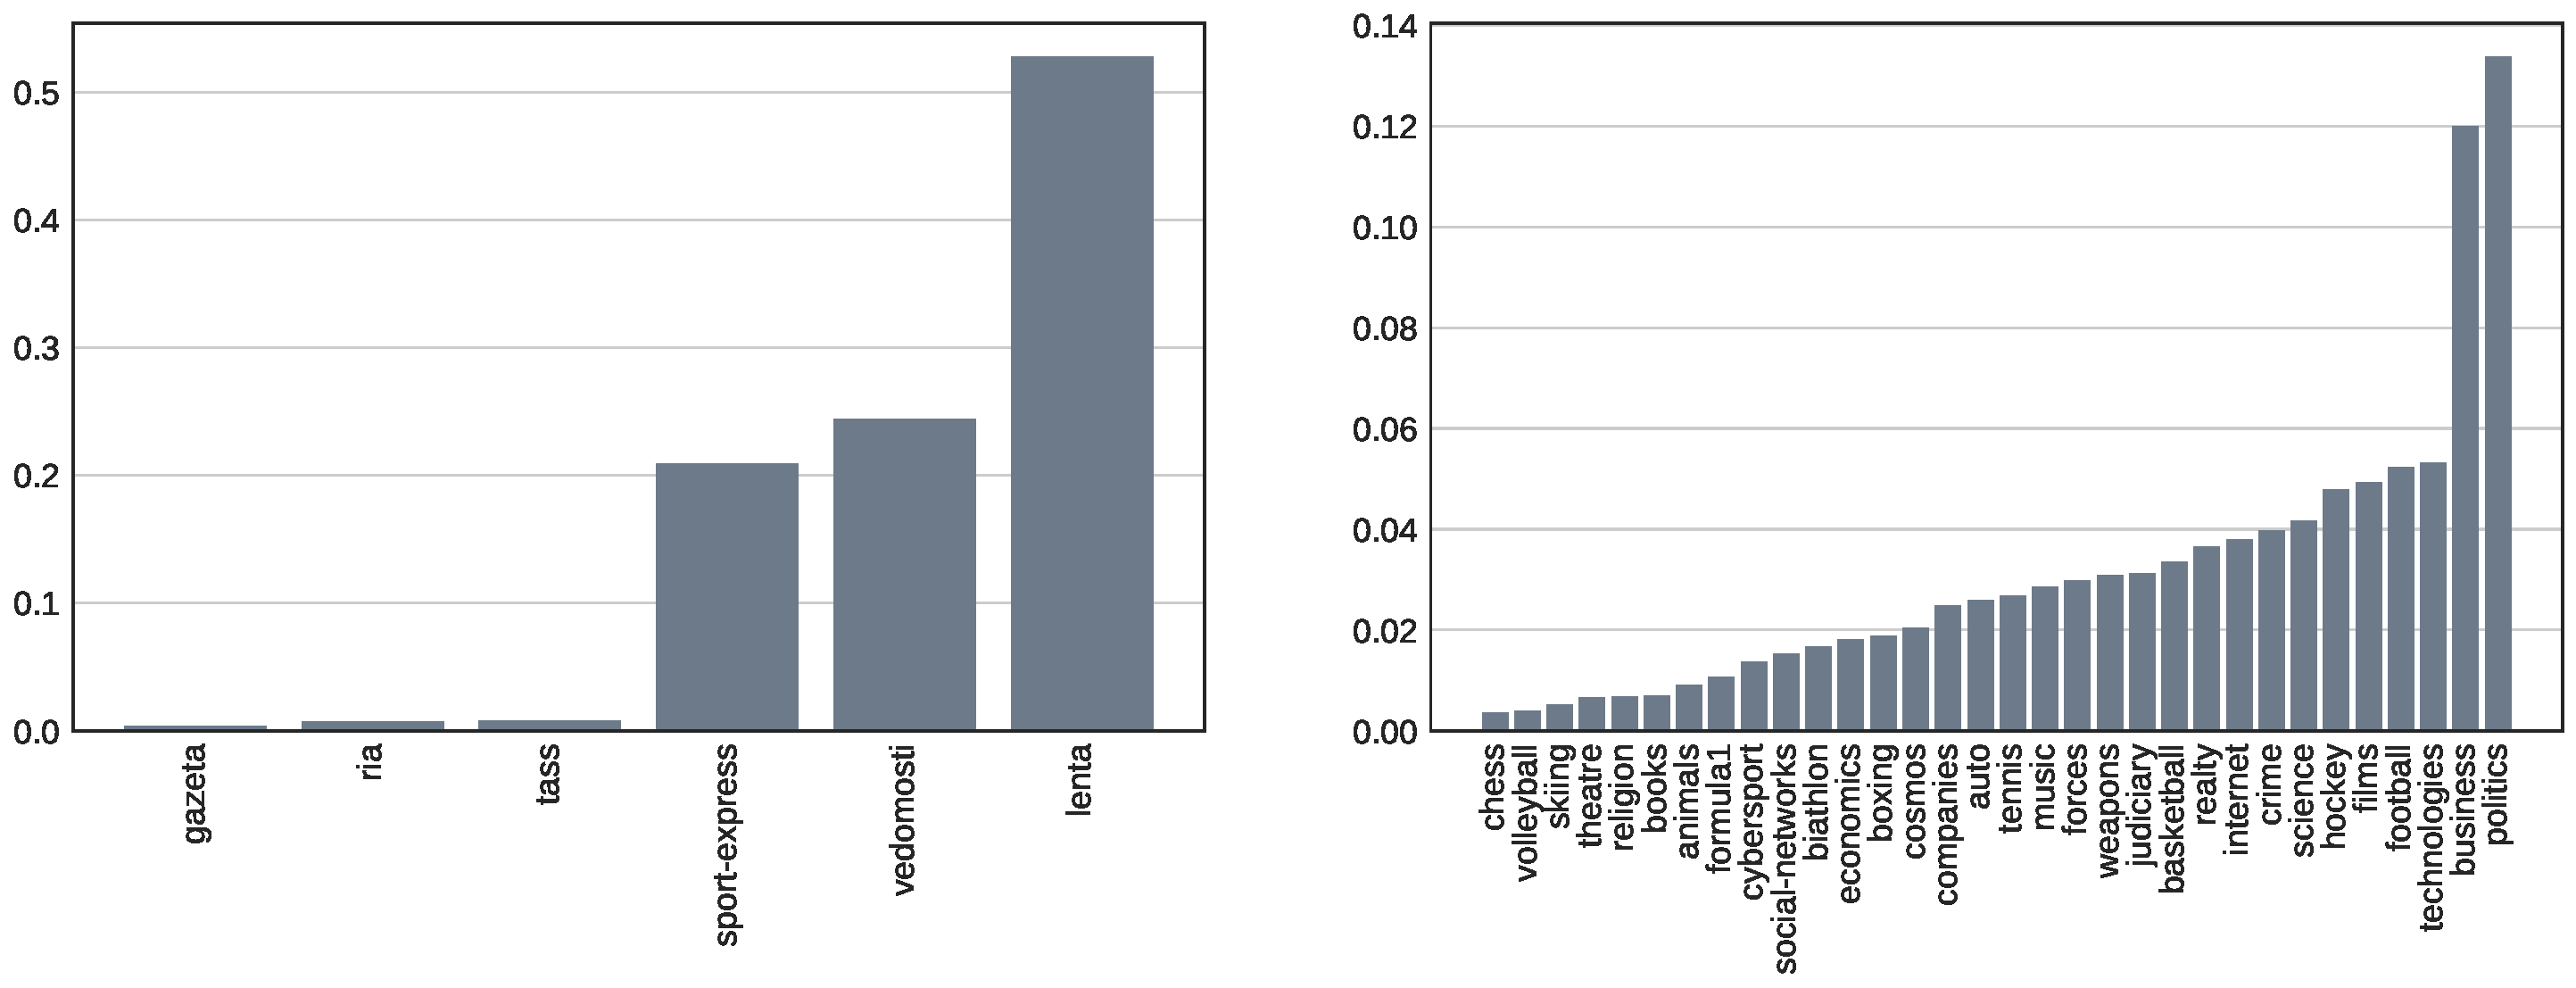
\includegraphics[width=1\textwidth]{media_topi_distr.pdf}
	\caption{Распределение СМИ и тем в данных}
	\label{media_topic_distr}
\end{figure}

%\lipsum[3-4]
\subsection{Препроцессинг новостных статей}
Препроцессинг является одной из важнейших стадий анализа данных. В данной работе, обработка данных начинается уже
на этапе получения новостей: из них удаляются все лишние HTML, JSON и XML теги.

Основной конвеер обработки данных состоит из нескольких последовательных этапов:
\begin{enumerate}
	\item Приведение текста в нижний регистр.
	\item Удаление чисел и символов пунктуации. Дефис сохраняется.
	\item Удаление стоп-слов. В данный набор входят наиболее часто употребляемые слова русского и английского языков,
	а также названия новостных агентств (<<лента>>, <<тасс>>, <<риа>> и т.д.), сохранение которых приводит к переобучению моделей.
	\item Лемматизация каждого слова с помощью библиотеки MyStem\footnote{\url{https://tech.yandex.ru/mystem/}}.
\end{enumerate}
Исходный код конвеера можно найти в приложении. %TODO: добавить ссылку

%\lipsum[3-4]
\section{Классификация новостных статей}
%\lipsum[3-4]
\subsection{Линейная модель на TF-IDF признаках}
%\lipsum[3-4]
\subsection{Градиентный бустинг деревьев на word2vec}
%\lipsum[3-4]
\section{Агрегация новостных статей}
\subsection{Кластеризация с помощью алгоритмов машинного обучения}
\subsection{Объединение в связные компоненты графа}
%\lipsum[3-4]
\section{Разработка веб-приложения}
\subsection{Back-end часть}
\subsection{Front-end часть}
%\lipsum[3-4]
\section{Заключение}
%\lipsum[3-5]

\bibliography{biblio}
 % Список литературы

\setcounter{secnumdepth}{0}
\section{Приложение}
%\lipsum[3-5]

\end{document}